%
% File acl2014.tex
%
% Contact: koller@ling.uni-potsdam.de, yusuke@nii.ac.jp
%%
%% Based on the style files for ACL-2013, which were, in turn,
%% Based on the style files for ACL-2012, which were, in turn,
%% based on the style files for ACL-2011, which were, in turn, 
%% based on the style files for ACL-2010, which were, in turn, 
%% based on the style files for ACL-IJCNLP-2009, which were, in turn,
%% based on the style files for EACL-2009 and IJCNLP-2008...
%% Based on the style files for EACL 2006 by 
%%e.agirre@ehu.es or Sergi.Balari@uab.es
%% and that of ACL 08 by Joakim Nivre and Noah Smith

\documentclass[11pt]{article}
\usepackage{acl2014}
\usepackage{times}
\usepackage{url}
\usepackage{latexsym}
\usepackage{amsmath}

\usepackage[usenames,dvipsnames,svgnames,table]{xcolor}
\usepackage{soul}

\usepackage{algorithm}
\usepackage[noend]{algpseudocode}
\usepackage{graphicx}
\usepackage{caption}
\usepackage{subcaption}

\usepackage{tikz-dependency}

\usepackage[usenames,dvipsnames,svgnames,table]{xcolor}  % allows better color names
\usepackage{todonotes}   % insert [disable] to disable all notes
% Note that these macros accept optional arguments such as 
% [size=\small,bordercolor=red].
\newcommand{\Note}[4][]{\todo[author=#2,color=#3,fancyline,#1]{#4}}
\newcommand{\noteJH}[2][]{\Note[#1]{MRG}{blue!40}{#2}}
\newcommand{\noteJE}[2][]{\Note[#1]{JE}{green!40}{#2}}   
\newcommand{\notewho}[3][]{\Note[#1]{#2}{orange!40}{#3}}  % extra arg with miscellaneous author
\newcommand{\NoteJH}[2][]{\noteJH[inline,#1]{#2}}
\newcommand{\NoteJE}[2][]{\noteJE[inline,#1]{#2}}
\newcommand{\Notewho}[3][]{\notewho[inline,#1]{#2}{#3}}  % extra arg with miscellaneous author

\title{Deriving Multi-Headed Projective Dependency Parses \\ from Link Grammar Parses}
% Oriented link grammar: Creating a multi-headed dependency corpus.

% \author{Juneki Hong and Jason Eisner\\
%   Department of Computer Science \\
%   Johns Hopkins University \\
%   Baltimore, MD 21218, USA \\ 
%   {\tt \{juneki,jason\}@cs.jhu.edu} \\
% }

\date{}

\begin{document}
\maketitle

\begin{abstract}
Under multi-headed dependency grammar, a parse is a DAG rather than a tree.  Such formalisms can be more syntactically and semantically expressive.  However, there are few multi-headed corpora at present, particularly for the projective case, so it is hard to investigate the benefit of such parsers or to work on making them faster or more accurate.  To fill this gap, we observe that link grammar produces {\em undirected} projective graphs.  
% OLD
% ... produces parses that are similar to multi-headed projective dependency parses, except that the links are undirected. 
We use Integer Linear Programming to assign consistent directions to the labeled links in a corpus of !!! \noteJE{fill in the number} parses produced by the Link Grammar Parser, which has broad-coverage hand-written grammars of English, Russian, and more. \noteJE{what statistics does it use?} We find that such directions can indeed be consistently assigned in a way that yields valid multi-headed dependency parses. The resulting parses in English appear reasonably linguistically plausible, although they are not in general consistent with CoNLL-style parses of the same sentences; we discuss the differences.  We also report on the convergence of our ILP method to a stable annotation scheme as the corpus size increases.
\end{abstract}


\section{Introduction}
\todo{Intro}
Projective dependency parsing is the task of mapping a sentence to a directed acyclic tree. Link parsing in contrast produces a multiheaded planar graph with undirected edges, where every edge has a label describing the relationship between two constituents in a parse. In this paper we explore whether these relationships include dependencies, and whether the multiheadedness of the link grammar offers additional dependency relationships not found in other corpora.

We will accomplish this by generating link parses using the AbiWord/CMU link grammar parser, learning a direction to every encountered link label type, and then using these assignments for all link tokens in the link parse corpus. We formulate an integer linear programming problem that will find the smallest set of assignments that will still produce dependency parses that are acyclic with all nodes reachable from the root.

From the ILP, we produce a dictionary of label-to-direction assignments. We publish this so that anyone can easily turn a link parse into a dependency parse.

Using the sentences of a dependency corpus as comparison, we find that the link parses do not wholly subsume dependency parses, and that the undirected links match roughly two thirds of the arcs in the conll dependency corpus. \todo{This is because...} 
Of the links that match a corresponding dependency arc we measure whether the direction we chose is the same as the original dependency data. 
Finally, we look to see that given a link label, whether the original conll label can be recovered.


%about 20\% 

%Kromann 2003 Danish dependency treebank\cite{kromann2003danish}
%McDonald and Pereira 2006\cite{McDonald2006}
%Sagae and Tsujii 2008\cite{Sagae2008}
%Gomez-Rodriguez and Nivre 2013\cite{gomez-rodriguez_divisible_2013}


Dependency parsing is the task of mapping a sentence to a projective (not always projective?) directed acyclic tree. Link parsing in contrast produces a multiheaded planar graph with undirected edges, where every edge has a label describing the relationship between two constituents in a parse. In this paper we explore whether these relationships include dependencies. To determine the directional dependencies within the link edge labels we will use integer linear programming, encoding the problem in the Zimpl little language \cite{Koch2004}. It turns out that the link parses roughly only match half of the conll dependency corpus. However this is because \todo{}. 

Some recent work has considered multi-headed ...

 by expressing the dependency of a word on multiple parents.

\cite{mcdonald-pereira-2006,buchkromann-2006,sagae-tsujii-2008,gomezrodriguez-nivre-2013}


 (check this) except for Buch-Kromann's work on Danish \cite{kromann-2003}

\NoteJE{discuss multiheadedness.  cite Kromann 2003's danish
  dependency treebank.  Prior work: McDonald and Pereira 2006, Sagae
  and Tsujii 2008, Gomez-Rodriguez and Nivre 2013.}
% http://aclweb.org/anthology/J/J13/J13-4002.pdf
% http://citeseerx.ist.psu.edu/viewdoc/download?doi=10.1.1.156.3938&rep=rep1&type=pdf


\section{Link Grammars}
Link grammars are a grammatical system equivalent to context-free grammars that assign linking requirements to every given word\cite{SleatorTemperly91}. A link parser then tries to satisfy all of these requirements for every word of a sentence while still maintaining planarity. The resulting links describe the relationships between constituents in a parse. 

The link grammar is based on a set of handwritten dictionaries. Instead of going through these dictionaries, we learned the grammar using an ILP. This approach also potentially allows us to analyze link grammar dictionaries other than English. \todo{explore other link grammar dictionaries} 


\section{Integer Linear Programming}
We formulated an ILP to assign directionality to all of the links in a set of link grammar parses, while still mandating that the resulting dependency parses are connected DAGs, with the nodes reachable from the root. 

In order to choose which direction the link labels are assigned, for every encountered label we generate two boolean label/direction variables correspending to left and right. Setting one of these variables to \textsc{true} allows only the specified direction for a label throughout all parses, and because we assign a directionality to every link type at least one of these variables must be set to true. Setting both variables would allow us to go in either direction.

Our ILP objective is to minimize the number of label/direction variables set to \textsc{true}, while still satisfying the acyclicity and reachability constraints. The encoding was written in the Zimpl little language \cite{Koch2004} and solved using the SCIP Optimization Suite\cite{achterberg2009scip}.

\todo{cite model minimization papers}

\begin{figure}
  \small
  \begin{align}
    \textsc{dir} &= \{\textsc{left}, \textsc{right}\} &\\ 
    \textsc{l} &\in \textsc{labels} & \\
    \textsc{m} &= \left|{\textsc{links}}\right| &\\
    \textsc{count}_{\textsc{l}, \textsc{dir}} &= \sum \textsc{link}_{\textsc{l},\textsc{dir}} &\\
    \textsc{count}_{\textsc{l}, \textsc{dir}} &= \textsc{m} \cdot \textsc{allowed}_{\textsc{l},\textsc{dir}} + \textsc{slack}_{\textsc{l}} &\\
    \textsc{cost}_{\textsc{l}} &= \frac{100}{\textsc{count}_{\textsc{l},\textsc{left}} + \textsc{count}_{\textsc{l},\textsc{right}}} &\\
    \text{minimize} &\sum_{\textsc{l}, \textsc{dir}} (\textsc{allowed}_{\textsc{l},\textsc{dir}}) + \textsc{cost}_{\textsc{l}} \cdot \sum_\textsc{l} \textsc{slack}_{\textsc{l}} &\\
    \text{subject to } &\forall_{i \in \textsc{sentence}}: \textsc{reachable}_{\textsc{root}, i} = \textsc{true} &\\
                       &\forall_{\substack{i,j \in \textsc{sentence} \\ i\neq j }}: \textsc{has\_cycle}_{i,j} = \textsc{false} &
  \end{align}
  \caption{\small The ILP formulation.}
\end{figure}

\subsection{Slack Hierarchy}

We introduced slack on the directional dependency variable tokens such that link types were allowed to deviate from the majority up to (1\% ?) of the time before the ILP would assign both directional dependency variables to true. This addressed noise in the link parser's label assignments, while still allowing for the possibility that both directions could still be assigned.

\todo{} We also introduced slack on the link types such that link types with the same coarse grained label would try and align the same way as the majority in the group, where the preceding capital letters of the link type denote the coarse grained label, while the subscript letters denote further information. This slack places a prior on rare or never-before seen link types to be assigned in the same way as other similar link types.

This slack hierarchy gave the ILP the flexibility to handle noise and novel link types while still trying to learn the overall link grammar.


\begin{equation}
  count_{L, \textsc{left}} = \sum_{a \in \textsc{ARCS}_L} left_a
\end{equation}
\begin{equation}
  count_{L, \textsc{left}} = \textsc{M} \cdot \textsc{allowed}_{L,\textsc{left}} + \textsc{slack}_{L}
\end{equation}
Where $L \in \textsc{LABELS}$, and $\textsc{M}$ is the size of the corpus.
The objective is:
\begin{equation}
  \min \sum_{L \in \textsc{LABELS} \atop \textsc{DIR} \in \{left, right\}} (\textsc{allowed}_{L,\textsc{DIR}}) \atop + \textsc{COST}(L) * \sum_L \textsc{slack}_L
\end{equation}
\begin{equation}
  \textsc{COST}(L) = \frac{100}{(\textsc{count}_{L,\textsc{left}} + \textsc{count}_{L,\textsc{right}})}
\end{equation}


\begin{algorithm}
\caption{ILP Encoding}\label{ILP}
\begin{algorithmic}[1]
%\Procedure{MyProcedure}{}

\State $\text{min} \sum_{l \in labels} allowed_L(l) + allowed_R(l)$
\State $\text{subject to}$
\State $\text{Acyclicity}$
\State $\text{All nodes reachable from the root.}$
\end{algorithmic}
\end{algorithm}

\subsection{Slack}
We introduced slack on the directional dependency variables such that the link types were allowed to deviate from the majority one percent of the time before the ILP would assign both directional dependency variables to true. This addressed noise in the link parser's label assignments, while still allowing for both directions to be assigned if needed.


\subsection{Stability of Results}
We measured how the solution changed over increasing numbers of processed sentences. 
Taking the solution to the largest run as the answer key, we measured how much the previous runs deviated from it. We measured the precision of whether the assignments in the smaller runs matched the assignments of the largest run and we measured the recall of whether the assignments in the largest run could be found in the smaller runs. 
\begin{figure}[ht!]
  \small
  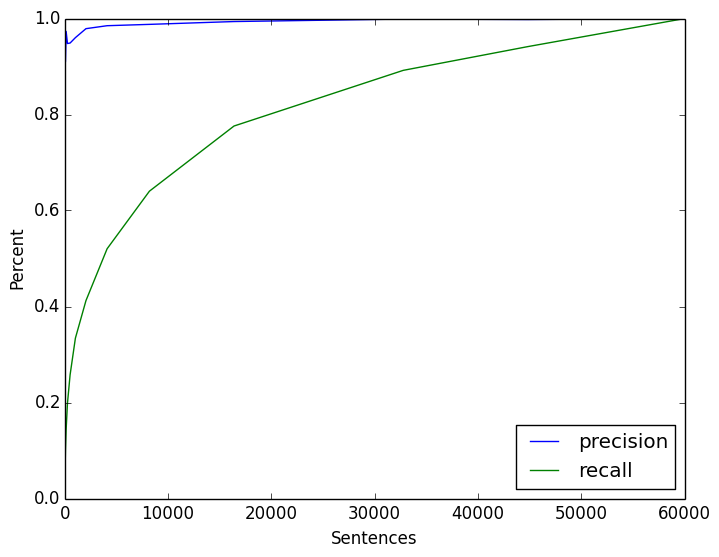
\includegraphics[width=\linewidth, keepaspectratio=true]{figure/precision_recall.png}
  \caption{\small Precision/recall of results of English sentences}
\end{figure}
We found that the precision values converged to 100\% while the recall values continued to grow throughout our data without converging. This indicates that the solutions of the previous runs were consistent with the largest run. However as the data grew, we would continue to encounter novel link types.



%\section{Other languages}




\section{Link Corpus Experiment and Results}
We ran the link parser on the english bnews corpus sentences. \footnote{We ignored the link parses that the link parser could not find suitable attachments and returned a disconnected graph. This happened for roughly 19\% of the sentences in the corpus.} 
From these parses we ran our ILP and generated directionalized multiheaded dependency data to compare with the original conll data.

\begin{figure}[ht!]
  \centering
  \small
  	\begin{tabular}{|l|l|}
		\hline
		Original number of sentences in conll corpus & 4096\\ 
		\hline
		Sentences after discarding disconnected parses & 3303\\ 
		\hline
		Sentences used for experiment and analysis & 2969\\ 
		\hline
	\end{tabular}

  \caption{\small Of the sentences used for this experiment section, about 0.00\%
    had at least one dropped word, and about 78.10\%
    had at least one multiheaded word}
\end{figure}



Compared to the original conll data, the link parses match about half the conll arcs in location and directionality. The mismatches in the other half can be accounted for in the following ways.

\subsection{Blanks}
Whenever the link parser failed to recognize a word from its dictionary, it would skip it and fail to attach any links. This accounts for about 10\% of the mismatches.

\subsection{Directional Mismatches}
In about 25\% of the cases, the conll arc's corresponding link would be assigned the opposite direction.


\section{Discussion}


\begin{figure*}[ht!]
  \centering
  \begin{subfigure}[b]{0.3233\textwidth}
	\begin{dependency}
		\begin{deptext}
			{\scriptsize PR} \& {\scriptsize VB} \& {\scriptsize RB} \& {\scriptsize VB} \& {\scriptsize .} \\
			it \& did \& n't \& work \& . \\
			- \& v-d \& - \& v \& - \\
		\end{deptext}
		\deproot[edge above, edge style = {blue, dotted}]{2}{\small ROOT}
		\depedge[edge below, edge style = {red, ultra thick}]{1}{2}{Ss}
		\depedge[edge above, edge style = {blue, thick}]{2}{1}{\small SBJ}
		\depedge[edge below, edge style = {red, thick}]{2}{3}{N}
		\depedge[edge above, edge style = {blue, thick}]{2}{3}{\small VMOD}
		\depedge[edge below, edge style = {red, thick}]{2}{4}{I*d}
		\depedge[edge above, edge style = {blue, thick}]{2}{4}{\small VC}
		\depedge[edge above, edge style = {blue, dotted}]{2}{5}{\small P}
		\deproot[edge below, edge style = {red, dotted}]{1}{Wd}
		\deproot[edge below, edge style = {orange, ultra thick}]{4}{WV}
		\deproot[edge below, edge style = {red, dotted}]{5}{Xp}
	\end{dependency}
\end{subfigure}
\begin{subfigure}[b]{0.3233\textwidth}
	\begin{dependency}
		\begin{deptext}
			{\scriptsize DT} \& {\scriptsize NN} \& {\scriptsize VB} \& {\scriptsize JJ} \& {\scriptsize .} \\
			the \& reason \& is \& simple \& . \\
			- \& n \& v \& a \& - \\
		\end{deptext}
		\deproot[edge below, edge style = {red, thick}]{3}{WV}
		\deproot[edge above, edge style = {blue, thick}]{3}{\small ROOT}
		\depedge[edge below, edge style = {red, thick}]{3}{2}{Ss*t}
		\depedge[edge above, edge style = {blue, thick}]{3}{2}{\small SBJ}
		\depedge[edge below, edge style = {red, thick}]{3}{4}{Paf}
		\depedge[edge above, edge style = {blue, thick}]{3}{4}{\small VMOD}
		\depedge[edge above, edge style = {blue, dotted}]{3}{5}{\small P}
		\depedge[edge below, edge style = {red, thick}]{2}{1}{D*u}
		\depedge[edge above, edge style = {blue, thick}]{2}{1}{\small NMOD}
		\deproot[edge below, edge style = {orange, ultra thick}]{2}{Wd}
		\deproot[edge below, edge style = {red, dotted}]{5}{Xp}
	\end{dependency}
\end{subfigure}
\begin{subfigure}[b]{0.3233\textwidth}
	\begin{dependency}
		\begin{deptext}
			{\scriptsize DT} \& {\scriptsize NN} \& {\scriptsize VB} \& {\scriptsize RB} \& {\scriptsize .} \\
			the \& judge \& wrote \& again \& . \\
			- \& n \& v-d \& - \& - \\
		\end{deptext}
		\deproot[edge below, edge style = {red, thick}]{3}{WV}
		\deproot[edge above, edge style = {blue, thick}]{3}{\small ROOT}
		\depedge[edge below, edge style = {red, thick}]{3}{2}{Ss}
		\depedge[edge above, edge style = {blue, thick}]{3}{2}{\small SBJ}
		\depedge[edge below, edge style = {red, thick}]{3}{4}{MVa}
		\depedge[edge above, edge style = {blue, thick}]{3}{4}{\small ADV}
		\depedge[edge above, edge style = {blue, dotted}]{3}{5}{\small P}
		\depedge[edge below, edge style = {red, thick}]{2}{1}{Ds}
		\depedge[edge above, edge style = {blue, thick}]{2}{1}{\small NMOD}
		\deproot[edge below, edge style = {orange, ultra thick}]{2}{Wd}
		\deproot[edge below, edge style = {red, dotted}]{5}{Xp}
	\end{dependency}
\end{subfigure}


  \caption{Example Sentences}
\end{figure*}

\todo{more in the appendix ...}

We should acknowledge that another option would be to post-process either CoNLL parses or our link parses to automatically add more multi-heading, e.g., to handle control phenomena ("John wants to skip" or "Jane ran for office in order to change the tax laws" should have John/Jane be the subject of two verbs).  However, that requires per-language 



\section{Future Work}

\subsection{Slack Hierarchy}
We would like to introduce slack on the link grammar types such that link types with the same coarse grained label would try and align the same way as the majority in the group, where the preceding capital letters of the link type denote the coarse grained label, while the subscript letters denote further information. This slack would place a prior on rare or never-before seen link types to be assigned in the same way as other similar link types. We think that this will give the ILP better flexibility to handle noise and novel link types while still trying to learn the overall link grammar.





\section{Related Work}



\bibliographystyle{acl2014}
\bibliography{LinksToDAG}





\clearpage
\appendix
\section{English Link Types}

\todo[inline]{A table here that lists each link grammar type together with its
  count, its allowed direction(s), its percentage of majority
  directions by token, and its most common corresponding CoNLL tags
  with percentages.  Readers could cut-and-paste this data to make a 
  cheap post-processor for LG parses.}

\section{Sample English Parses}

\todo[inline]{Show a bunch of English sentences with CoNLL vs.\@ link parses.
  Explain how they were selected and how the results are colorized etc.}

\end{document}
